\documentclass[a4paper,12pt]{article}
\usepackage[utf8]{inputenc}
\usepackage{amsmath}
\usepackage{amssymb}
\usepackage{graphicx}
\usepackage{geometry}
\usepackage{tikz}
\usepackage{pgfplots}
\pgfplotsset{width=9cm, compat=1.9}
\usepackage{multicol}
\usepackage{array}
\setlength{\columnsep}{1cm}
\usepackage[inline]{enumitem}
\usepackage{setspace}
\usepackage{subcaption}
\usepackage{array}
\newcolumntype{L}[1]{>{\raggedright\let\newline\\\arraybackslash\hspace{0pt}}m{#1}}
\newcolumntype{C}[1]{>{\centering\let\newline\\\arraybackslash\hspace{0pt}}m{#1}}
\newcolumntype{R}[1]{>{\raggedleft\let\newline\\\arraybackslash\hspace{0pt}}m{#1}}
\usepackage{tcolorbox}
\renewcommand{\arraystretch}{1.5}
\geometry{a4paper, top=1.25cm,bottom=2cm,right=2cm,left=2cm}
\setlength\parindent{0pt}
%------------------------------------------------------------------
% line drawer number of lines, line spacing, line width
\newcommand\lineControl[3]{
	\vspace{0.025cm}\begin{tikzpicture}
	\draw[white](0,-0.25); 
	\foreach \y in {1,...,#1}{
		\draw[line width=0mm](0,-\y*#2)--(#3,-\y*#2);
	}
	\end{tikzpicture}\vspace{0cm}
}
%------------------------------------------------------------------
\newcommand{\lThick}{0.1 mm}
%------------------------------------------------------------------
\newcommand\sumproduct[5]{
	\begin{tikzpicture}[scale=0.6]
	\draw[white](-4.75,-2.75)rectangle(4.75,5);
	\draw[](-4.5,4.5)node[right, yshift=-0.2cm]{\footnotesize \textbf{#5)}};
	\draw[](-4,0)rectangle(0,2);
	\draw[](0,0)rectangle(4,2);
	\draw[](-2,2)rectangle(2,4);
	\draw[](-2,-2)rectangle(2,0);
	\draw[](0,-1)node[]{#1};
	\draw[](0,3)node[]{#2};
	\draw[](-2,1)node[]{#3};
	\draw[](2,1)node[]{#4};
	\draw[](-4,3)node[right]{\tiny Product:};
	\draw[](-4,-1)node[right]{\tiny Sum:};
	\end{tikzpicture}
}
%------------------------------------------------------------------
\begin{document}
\section{Homework sheet}
\begin{flushright}
Name\rule{8cm}{\lThick}
\end{flushright} 
\begin{enumerate}
\item Identify the prime numbers in the following sets:
\begin{enumerate}
\item 	$\{3,6,10,13,18,21\}$
\item	$\{40,41,42,45,46,47,49\}$
\item	$\{87,89,91,93,95,97\}$
\end{enumerate}
\item Find the prime factors of: 
\begin{enumerate}
	\item $14$
	\item $39$
	\item $77$
\end{enumerate}
\item Draw factor trees for the following numbers and write the numbers as a product of prime factors.
\begin{enumerate}
	\item $120$
	\item $94$
	\item $630$
\end{enumerate}
\item ( please show working for each ) Find the Highest Common Factor of:
\begin{enumerate}
	\item $40$ and $64$
	\item $42$ and $56$
	\item $54$ and $78$
\end{enumerate}
\item ( please show working for each ) Find the Lowest Common Multiple of:
\begin{enumerate}
	\item $8$ and $12$
	\item $9$ and $15$
	\item $28$ and $35$
\end{enumerate}
\item 5678 has prime factors 2, 17, 167.
\begin{enumerate}
		\item Draw a factor tree for the number.
		\item Write a factor list for the number.
\end{enumerate} 
\item Carol is making lunch packs. She has 21 vegetarian sushi rolls and 35 rice and seaweed rolls . What is the maximum number of packs she can make and how many of each roll will be in a pack?
\item Mary can paint a house in 6 days and Miranda can paint a house in 9 days. Working together, how long will it take them to paint one house?
\end{enumerate}
\newpage
\lineControl{26}{1}{17}
\newpage
\lineControl{26}{1}{17}
\newpage
\section{Homework and class practice questions for the test}
\begin{flushright}
	Name\rule{8cm}{\lThick}
\end{flushright} 
\newcommand{\wdth}{2}
\newcommand{\hght}{1}
\begin{enumerate}
	\item Definitions
	\begin{enumerate}
		\item What is the definition of a \textbf{factor}?
		\item What is the definition of a \textbf{prime number}?
	\end{enumerate}
	\item In each set of Whole Numbers, circle the prime numbers.\\
	(if 2,3,5 and 7 don't divide into them then they will be prime).
	\begin{enumerate}
		\item \{10, 3, 21, 17, 15, 11, 16, 4, 2, 23\}
		\item \{65, 66, 67, 68, 69, 70, 71, 72, 73, 74\}
	\end{enumerate} 
	\item Make factor trees for the following numbers and write each number as a product of its prime factors.
	\begin{multicols}{4}
		\begin{enumerate}
			\item 100
			\item 120
			\item 164
		\end{enumerate}
	\end{multicols}
	\item Find the \textbf{Highest Common Factor} for the following pairs of numbers
\begin{multicols}{5}
	\begin{enumerate}
		\item 80, 52
		\item 96, 36
	\end{enumerate}
\end{multicols}
	\item Find the \textbf{Lowest Commmon Multiple} for the following pairs of numbers
	\begin{multicols}{5}
		\begin{enumerate}
			\item 12, 26
			\item 18, 33
		\end{enumerate}
	\end{multicols}
	\item Write factor lists for:
	\begin{multicols}{4}
		\begin{enumerate}
			\item 144
			\item 120
		\end{enumerate} 
	\end{multicols}
	\item Calculate the following
	\begin{multicols}{3}
		\begin{enumerate}
			\item $\displaystyle -17-20= $
			\item $\displaystyle -2-(-14)= $
			\item $\displaystyle -14+(-3)=$
			\item $\displaystyle -17\times (-3)=$
			\item $\displaystyle 15\div (-3)=$
			\item $\displaystyle 4\times (-8)=$
		\end{enumerate}
	\end{multicols}
	\item The two bricks below add to the brick above. Fill in the missing bricks:\\
	\begin{center}
		\begin{tikzpicture}
		\draw[black, thin] (0,0) rectangle (\wdth,\hght)node[midway]{$-5$};
		\draw[black, thin] (\wdth,0) rectangle (2*\wdth,\hght);
		\draw[black, thin] (2*\wdth,0) rectangle (3*\wdth,\hght)node[midway]{$-7$};
		\draw[black, thin] (\wdth/2,\hght) rectangle (3*\wdth/2,2*\hght)node[midway]{$6$};
		\draw[black, thin] (3*\wdth/2,\hght) rectangle (5*\wdth/2,2*\hght);
		\draw[black, thin] (\wdth,2*\hght) rectangle (2*\wdth,3*\hght);
		\end{tikzpicture}
	\end{center}
	\newpage
	\item The numbers in the circles \textbf{multiply} to give the number in the squares between them. Fill in the missing spaces:\\
	\begin{center}
		\begin{tikzpicture}
		\coordinate (A) at (0,0);
		\coordinate (B) at (3*\wdth,0);
		\coordinate (C) at (1.5*\wdth,4*\hght);
		\draw[black, thin] (A)--(B)--(C)--(A);
		\filldraw[draw=black,fill=white, thin] (A) circle[radius=0.6cm]node{$-3$};
		\filldraw[draw=black,fill=white, thin] (B) circle[radius=0.6cm]node{$-8$};
		\filldraw[draw=black,fill=white, thin] (C) circle[radius=0.6cm];
		\filldraw[draw=black,fill=white, thin] (0.75*\wdth-0.5,2*\hght-0.5) rectangle(0.75*\wdth+0.5,2*\hght+0.5)node[midway]{$15$};
		\filldraw[draw=black, fill=white, thin] (2.25*\wdth-0.5,2*\hght-0.5) rectangle(2.25*\wdth+0.5,2*\hght+0.5);
		\filldraw[draw=black,fill=white, thin] (1.5*\wdth-0.5,0-0.5) rectangle(1.5*\wdth+0.5,0+0.5);
		\end{tikzpicture}
	\end{center}
	\item (Difficult)Calculate the following
	\begin{multicols}{3}
		\begin{enumerate}
			\item $\displaystyle 4^{2}\div 2= $
			\item $\displaystyle -3\times -4\div (5+1)= $
			\item $\displaystyle  -2\times (5+-9)=$
			\item $\displaystyle (2^{5}+2)\times 3=$
			\item $\displaystyle (-2+5)\times \sqrt{36}=$
			\item $\displaystyle 4^{4}\times 0.5+\sqrt{121}=$
		\end{enumerate}
	\end{multicols}
	\item Write the following Decimals as Fractions
	\begin{multicols}{4}
		\begin{enumerate}
			\item $\displaystyle 0.46$
			\item $\displaystyle 0.968$
			\item $\displaystyle 0.\dot{4}$
			\item $\displaystyle 0.\dot{8}$
		\end{enumerate}
	\end{multicols}
\item Write the following as fractions:
	\begin{multicols}{4}
	\begin{enumerate}
		\item $\displaystyle \left(\frac{1}{2} \right)^5$
		\item $\displaystyle \left(\frac{1}{3} \right)^2$
		\item $\displaystyle 5^{-3}$
		\item $\displaystyle 10^{-2}$
	\end{enumerate}
\end{multicols}
	\item Simplify:
	\begin{multicols}{4}
		\begin{enumerate}
			\item $\displaystyle \sqrt{2}\times \sqrt{3}$
			\item $\displaystyle \sqrt{5}\times \sqrt{6}$

		\end{enumerate}
	\end{multicols}
	\item Calculate:
	\begin{multicols}{4}
		\begin{enumerate}
			\item $\displaystyle  \sqrt{36}$
			\item $\displaystyle \sqrt{64}$
			\item $\displaystyle \sqrt{81}$
			\item $\displaystyle \sqrt{121}$
		\end{enumerate}
	\end{multicols}
\end{enumerate}
\lineControl{7}{1}{17}
\newpage
\lineControl{26}{1}{17}
\newpage
\lineControl{26}{1}{17}
\newpage
\section{Homework and class practice questions for the test}
\begin{flushright}
	Name\rule{8cm}{\lThick}
\end{flushright} 

\begin{enumerate}
		\item Find the \textbf{Lowest Commmon Multiple} for the following pairs of numbers
	\begin{multicols}{5}
		\begin{enumerate}
			\item 9, 24
		\end{enumerate}
	\end{multicols}

		\item Calculate the following
	\begin{multicols}{3}
		\begin{enumerate}
			\item $\displaystyle -7+13= $
			\item $\displaystyle 5-(-10)= $
			\item $\displaystyle 14+(-18)=$
			\item $\displaystyle 9\times (-6)=$
			\item $\displaystyle -35\div (-5)=$
			\item $\displaystyle -4\times (-6)=$
		\end{enumerate}
	\end{multicols}
	\item Find the \textbf{Highest Common Factor} for the following pairs of numbers
\begin{multicols}{5}
	\begin{enumerate}
		\item 110, 90
	\end{enumerate}
\end{multicols}
	\item In each set of Whole Numbers, circle the prime numbers.\\
	(if 2,3,5 and 7 don't divide into them then they will be prime).
	\begin{enumerate}
		\item \{5, 83, 19, 57, 11, 93, 47,97, 51, 39\}
	\end{enumerate} 
	\item Make factor trees for the following numbers and write each number as a product of its prime factors.
	\begin{multicols}{4}
		\begin{enumerate}
			\item 196
		\end{enumerate}
	\end{multicols}
\item Write factor lists for:
	\begin{multicols}{4}
		\begin{enumerate}
			\item 96
		\end{enumerate} 
	\end{multicols}

	\item The two bricks below add to the brick above. Fill in the missing bricks:\\
	\begin{center}
		\begin{tikzpicture}
		\draw[black, thin] (0,0) rectangle (\wdth,\hght)node[midway]{};
		\draw[black, thin] (\wdth,0) rectangle (2*\wdth,\hght)node[midway]{$-8$};
		\draw[black, thin] (2*\wdth,0) rectangle (3*\wdth,\hght)node[midway]{};
		\draw[black, thin] (\wdth/2,\hght) rectangle (3*\wdth/2,2*\hght)node[midway]{$-1$};
		\draw[black, thin] (3*\wdth/2,\hght) rectangle (5*\wdth/2,2*\hght);
		\draw[black, thin] (\wdth,2*\hght) rectangle (2*\wdth,3*\hght)node[midway]{$-5$};;
		\end{tikzpicture}
	\end{center}
	\newpage
	\item The numbers in the circles \textbf{multiply} to give the number in the squares between them. Fill in the missing spaces:\\
	\begin{center}
		\begin{tikzpicture}
		\coordinate (A) at (0,0);
		\coordinate (B) at (3*\wdth,0);
		\coordinate (C) at (1.5*\wdth,4*\hght);
		\draw[black, thin] (A)--(B)--(C)--(A);
		\filldraw[draw=black,fill=white, thin] (A) circle[radius=0.6cm]node{$2$};
		\filldraw[draw=black,fill=white, thin] (B) circle[radius=0.6cm]node{$-1$};
		\filldraw[draw=black,fill=white, thin] (C) circle[radius=0.6cm];
		\filldraw[draw=black,fill=white, thin] (0.75*\wdth-0.5,2*\hght-0.5) rectangle(0.75*\wdth+0.5,2*\hght+0.5)node[midway]{$-12$};
		\filldraw[draw=black, fill=white, thin] (2.25*\wdth-0.5,2*\hght-0.5) rectangle(2.25*\wdth+0.5,2*\hght+0.5);
		\filldraw[draw=black,fill=white, thin] (1.5*\wdth-0.5,0-0.5) rectangle(1.5*\wdth+0.5,0+0.5);
		\end{tikzpicture}
	\end{center}
	\item (Difficult)Calculate the following
	\begin{multicols}{3}
		\begin{enumerate}
			\item $\displaystyle 4^{2}\times \sqrt{25}= $
			\item $\displaystyle -30\div -5\times (5-3)^{2}= $
			\item $\displaystyle  2\times (1+-5)^{2}=$
			\item $\displaystyle (2^{3}+1)\times \sqrt[3]{125}=$
			\item $\displaystyle -6^2=$
			\item $\displaystyle (-6)^2=$
		\end{enumerate}
	\end{multicols}
	\item Write the following Decimals as Fractions
	\begin{multicols}{4}
		\begin{enumerate}
			\item $\displaystyle 0.88$
			\item $\displaystyle 0.06$
			\item $\displaystyle 0.\dot{1}$
			\item $\displaystyle 0.\dot{7}$
		\end{enumerate}
	\end{multicols}
	\item Write the following as fractions:
	\begin{multicols}{4}
		\begin{enumerate}
			\item $\displaystyle 6^{-3}$
			\item $\displaystyle 6^{3}$
			\item $\displaystyle \left(\frac{1}{2} \right)^3$
			\item $\displaystyle \left(\frac{1}{2} \right)^{-3}$
		\end{enumerate}
	\end{multicols}
	\item Simplify:
	\begin{multicols}{4}
		\begin{enumerate}
			\item $\displaystyle \sqrt{18}\times \sqrt{2}$
			\item $\displaystyle \sqrt{10}\times \sqrt{10}$
			
		\end{enumerate}
	\end{multicols}
	\item Square numbers are made by multiplying the a number with itself. For example 9 is a square number because $3\times 3=9$.\\
	Starting with $1\times 1=1$, write out the first 10 square numbers.
\end{enumerate}
\lineControl{7}{1}{17}
\newpage
\lineControl{26}{1}{17}
\newpage
\lineControl{26}{1}{17}
\newpage
\begin{center}
	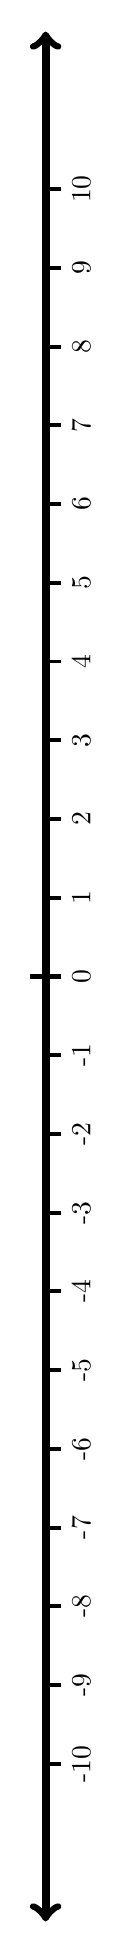
\begin{tikzpicture}[rotate = 90]
	\draw[black, line width=1mm, ->](0,0)--(12,0);
	\draw[black, line width=1mm, ->](0,0)--(-12,0);
	\draw[black, ultra thick](0,-0.2)--(0,0.2);
	\foreach \x in {-10,-9,...,10}{
		\draw[black, line width=0.5mm](\x,0)--(\x,-0.2)node[right]{\rotatebox{90}{\x} };
	}
	\end{tikzpicture}\hspace{5cm}
		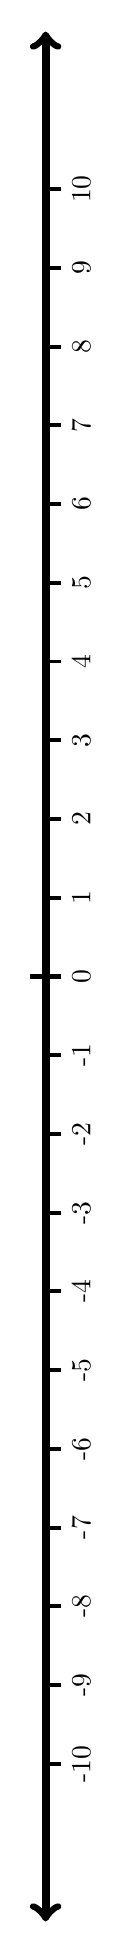
\begin{tikzpicture}[rotate = 90]
	\draw[black, line width=1mm, ->](0,0)--(12,0);
	\draw[black, line width=1mm, ->](0,0)--(-12,0);
	\draw[black, ultra thick](0,-0.2)--(0,0.2);
	\foreach \x in {-10,-9,...,10}{
		\draw[black, line width=0.5mm](\x,0)--(\x,-0.2)node[right]{\rotatebox{90}{\x} };
	}
	\end{tikzpicture}\hspace{5cm}
			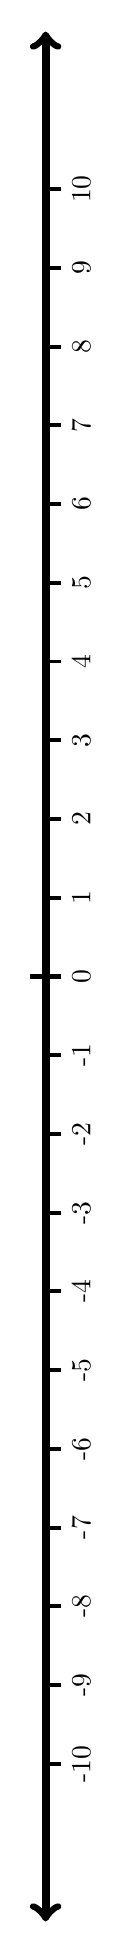
\begin{tikzpicture}[rotate = 90]
	\draw[black, line width=1mm, ->](0,0)--(12,0);
	\draw[black, line width=1mm, ->](0,0)--(-12,0);
	\draw[black, ultra thick](0,-0.2)--(0,0.2);
	\foreach \x in {-10,-9,...,10}{
		\draw[black, line width=0.5mm](\x,0)--(\x,-0.2)node[right]{\rotatebox{90}{\x} };
	}
	\end{tikzpicture}
\end{center}\vspace{0.5cm}
\newpage
With the number given, use the number line to divide it up into \textbf{equal} parts\\
Then write a multiplication to go with it.\\\\ 
Number is: 6\\\\
			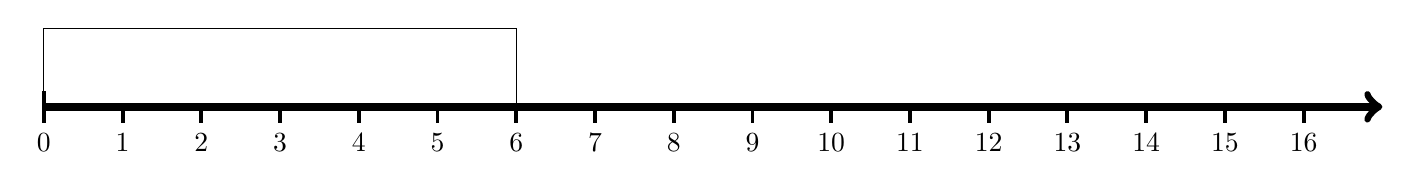
\begin{tikzpicture}[rotate = 0]
\draw[black, line width=0.1mm](0,0) rectangle (6,1);
\draw[black, line width=1mm, ->](0,0)--(17,0);
\draw[black, ultra thick](0,-0.2)--(0,0.2);
\foreach \x in {0,1,...,16}{
	\draw[black, line width=0.5mm](\x,0)--(\x,-0.2)node[below]{\rotatebox{00}{\x} };
}
\end{tikzpicture}\\\\
Multiplication is : $\underline{~~~~} \times \underline{~~~~} =6$\\\\\\
Number is: 8\\\\
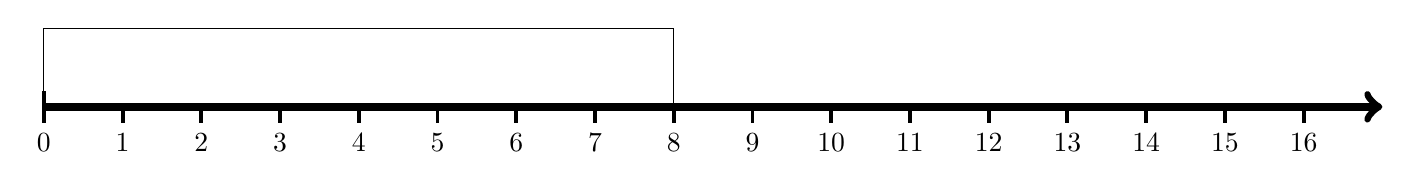
\begin{tikzpicture}[rotate = 0]
\draw[black, line width=0.1mm](0,0) rectangle (8,1);
\draw[black, line width=1mm, ->](0,0)--(17,0);
\draw[black, ultra thick](0,-0.2)--(0,0.2);
\foreach \x in {0,1,...,16}{
	\draw[black, line width=0.5mm](\x,0)--(\x,-0.2)node[below]{\rotatebox{00}{\x} };
}
\end{tikzpicture}\\\\
Multiplication is : $\underline{~~~~} \times \underline{~~~~} =8$\\\\\\
Number is: 9\\\\
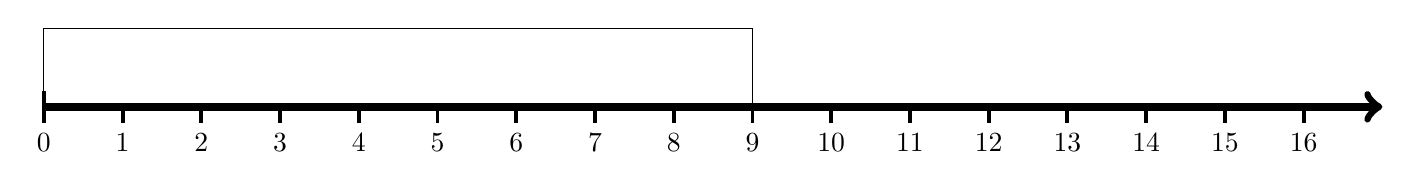
\begin{tikzpicture}[rotate = 0]
\draw[black, line width=0.1mm](0,0) rectangle (9,1);
\draw[black, line width=1mm, ->](0,0)--(17,0);
\draw[black, ultra thick](0,-0.2)--(0,0.2);
\foreach \x in {0,1,...,16}{
	\draw[black, line width=0.5mm](\x,0)--(\x,-0.2)node[below]{\rotatebox{00}{\x} };
}
\end{tikzpicture}\\\\
Multiplication is : $\underline{~~~~} \times \underline{~~~~} =8$\\\\\\
Number is: 10\\\\
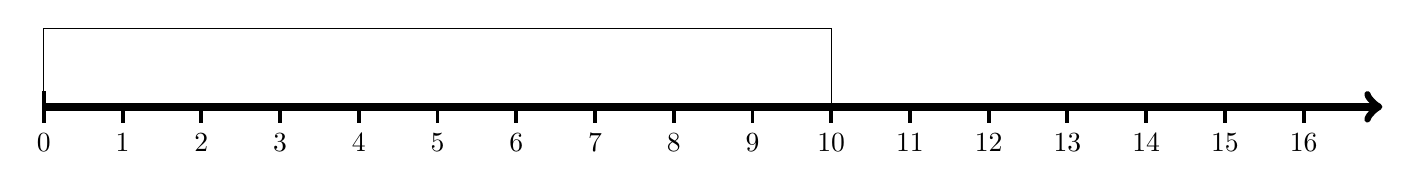
\begin{tikzpicture}[rotate = 0]
\draw[black, line width=0.1mm](0,0) rectangle (10,1);
\draw[black, line width=1mm, ->](0,0)--(17,0);
\draw[black, ultra thick](0,-0.2)--(0,0.2);
\foreach \x in {0,1,...,16}{
	\draw[black, line width=0.5mm](\x,0)--(\x,-0.2)node[below]{\rotatebox{00}{\x} };
}
\end{tikzpicture}\\\\
Multiplication is : $\underline{~~~~} \times \underline{~~~~} =10$\\\\\\
Number is: 12\\\\
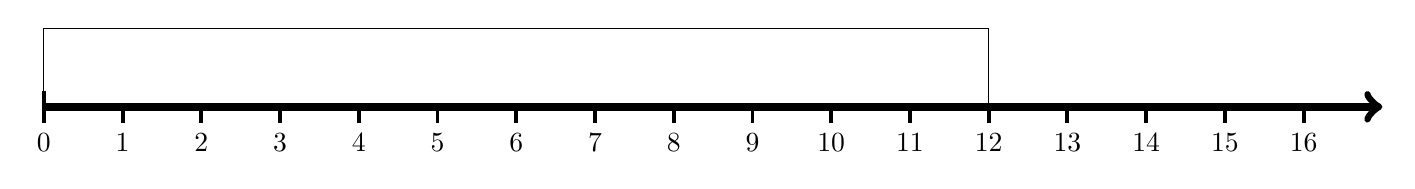
\begin{tikzpicture}[rotate = 0]
\draw[black, line width=0.1mm](0,0) rectangle (12,1);
\draw[black, line width=1mm, ->](0,0)--(17,0);
\draw[black, ultra thick](0,-0.2)--(0,0.2);
\foreach \x in {0,1,...,16}{
	\draw[black, line width=0.5mm](\x,0)--(\x,-0.2)node[below]{\rotatebox{00}{\x} };
}
\end{tikzpicture}\\\\
Multiplication is : $\underline{~~~~} \times \underline{~~~~} =12$\\\\\\
\newpage
Number is: 12  (chose a different way of dividing up)\\\\
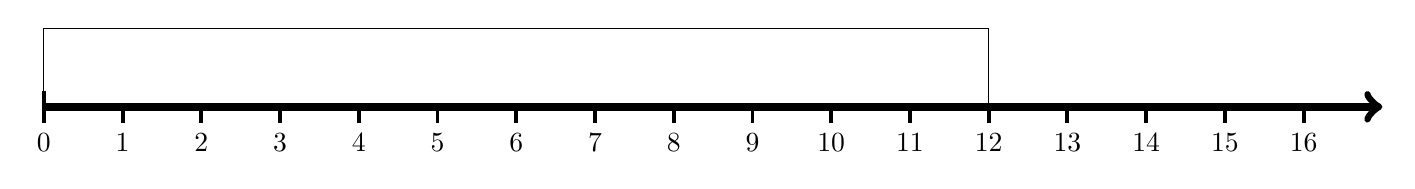
\begin{tikzpicture}[rotate = 0]
\draw[black, line width=0.1mm](0,0) rectangle (12,1);
\draw[black, line width=1mm, ->](0,0)--(17,0);
\draw[black, ultra thick](0,-0.2)--(0,0.2);
\foreach \x in {0,1,...,16}{
	\draw[black, line width=0.5mm](\x,0)--(\x,-0.2)node[below]{\rotatebox{00}{\x} };
}
\end{tikzpicture}\\\\
Multiplication is : $\underline{~~~~} \times \underline{~~~~} =12$\\\\

Number is: 14 \\\\
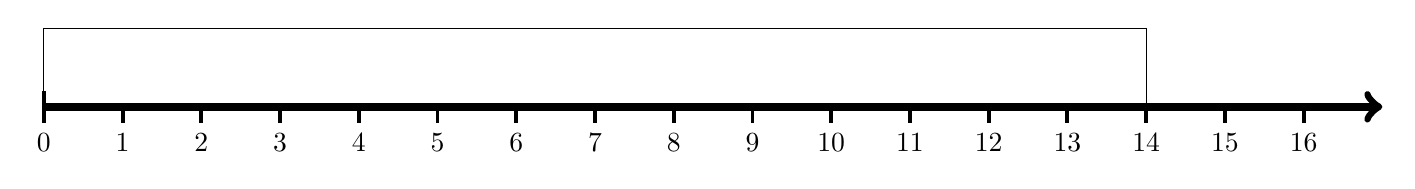
\begin{tikzpicture}[rotate = 0]
\draw[black, line width=0.1mm](0,0) rectangle (14,1);
\draw[black, line width=1mm, ->](0,0)--(17,0);
\draw[black, ultra thick](0,-0.2)--(0,0.2);
\foreach \x in {0,1,...,16}{
	\draw[black, line width=0.5mm](\x,0)--(\x,-0.2)node[below]{\rotatebox{00}{\x} };
}
\end{tikzpicture}\\\\
Multiplication is : $\underline{~~~~} \times \underline{~~~~} =14$\\\\\\
Number is: 15  \\\\
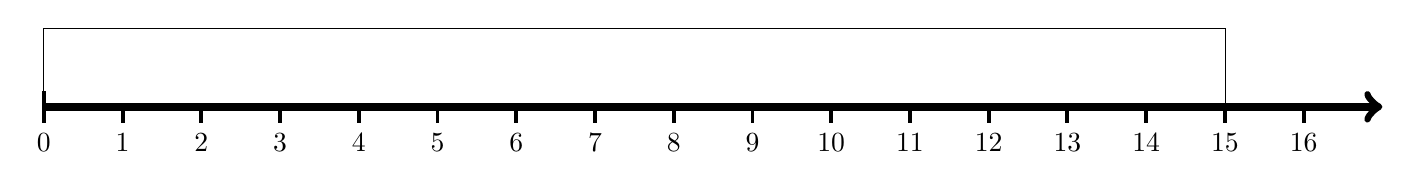
\begin{tikzpicture}[rotate = 0]
\draw[black, line width=0.1mm](0,0) rectangle (15,1);
\draw[black, line width=1mm, ->](0,0)--(17,0);
\draw[black, ultra thick](0,-0.2)--(0,0.2);
\foreach \x in {0,1,...,16}{
	\draw[black, line width=0.5mm](\x,0)--(\x,-0.2)node[below]{\rotatebox{00}{\x} };
}
\end{tikzpicture}\\\\
Multiplication is : $\underline{~~~~} \times \underline{~~~~} =15$\\\\\\
Number is: 16  \\\\
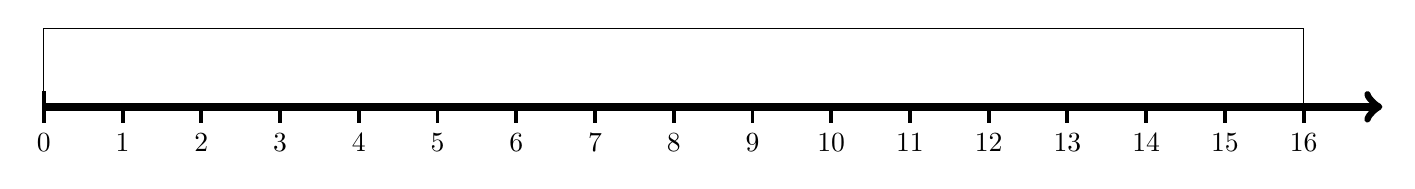
\begin{tikzpicture}[rotate = 0]
\draw[black, line width=0.1mm](0,0) rectangle (16,1);
\draw[black, line width=1mm, ->](0,0)--(17,0);
\draw[black, ultra thick](0,-0.2)--(0,0.2);
\foreach \x in {0,1,...,16}{
	\draw[black, line width=0.5mm](\x,0)--(\x,-0.2)node[below]{\rotatebox{00}{\x} };
}
\end{tikzpicture}\\\\
Multiplication is : $\underline{~~~~} \times \underline{~~~~} =16$\\\\
\newpage

\newcommand\numLine[1]{
Number is: #1  \\\\
\begin{tikzpicture}[rotate = 0]
\draw[black, line width=0.1mm](0,0) rectangle (#1/2,1);
\draw[black, line width=1mm, ->](0,0)--(17,0);
\draw[black, ultra thick](0,-0.2)--(0,0.2);
\foreach \x in {0,2,...,32}{
	\draw[black, line width=0.5mm](\x/2,0)--(\x/2,-0.2)node[below]{\rotatebox{00}{\x} };
}
\foreach \x in {0,1,...,#1}{
	\draw[red, line width=0.1mm](\x/2,0)--(\x/2,1);
}
\foreach \x in {0,2,...,#1}{
	\draw[blue, line width=0.1mm](\x/2,0)--(\x/2,1);
}
\end{tikzpicture}\\\\
Multiplication is : $\underline{~~~~} \times \underline{~~~~} =#1$\\\\\\
}
With the number given, use the number line to divide it up into \textbf{equal} parts\\
Then write a multiplication to go with it.\\\\
\numLine{12}
\numLine{14}
\numLine{16}
\numLine{18}
\numLine{20}
\newpage
\numLine{22}
\numLine{24}
\numLine{26}
\numLine{28}
\numLine{30}
\newpage
Work out (use number grid or steps):
\begin{enumerate}
	\item \begin{enumerate}
	\item ~~~~~$ 2 \times 2 =$
	\item ~~~~~$ 2 \times 2 \times 2 =$  
	\item ~~~~~$ 2 \times 2 \times 2 \times 2 =$
	\item ~~~~~$ (2 \times 2 \times 2 ) \times (2 \times 2) =$
	\item ~~~~~$ (2 \times 2 \times 2) \times (2 \times 2 \times 2) =$
\end{enumerate}
	\item \begin{enumerate}
	\item ~~~~~$ 3 \times 3 =$
	\item ~~~~~$ 3 \times 3 \times 3 =$  
	\item ~~~~~$ (3 \times 3) \times (3 \times 3) =$
\end{enumerate}
	\item \begin{enumerate}
	\item ~~~~~$ 4 \times 4 =$
\end{enumerate}
	\item \begin{enumerate}
	\item ~~~~~$ 6 \times 6 =$
\end{enumerate}
	\item \begin{enumerate}
	\item ~~~~~$ 7 \times 7 =$
\end{enumerate}
\end{enumerate}

\begin{enumerate}
	\item \begin{enumerate}
		\item ~~~~~$ 10 + 10 =$
		\item ~~~~~$ 10 + 10 + 10 =$  
		\item ~~~~~$ 10 + 10 + 10 +10 =$
	\end{enumerate}
	\item \begin{enumerate}
		\item ~~~~~$ 4 \times 10 =$
		\item ~~~~~$ 5 \times 10 =$  
		\item ~~~~~$ 6 \times 10 + 5 =$
	\end{enumerate}
	\item \begin{enumerate}
		\item ~~~~~$ 2 \times 15 = 2 \times 10 + 2 \times 5 = $
	\end{enumerate}
	\item \begin{enumerate}
		\item ~~~~~$ 3 \times 15 = 3 \times 10 + 3 \times 5 =$
	\end{enumerate}
	\item \begin{enumerate}
		\item ~~~~~$ 4 \times 15 = 4 \times 10 + 4 \times 5 =$
	\end{enumerate}
\end{enumerate}




\end{document}